\documentclass[11pt,a4paper]{article}

\usepackage[utf8]{inputenc}
\usepackage[spanish]{babel}
\usepackage{amsmath}
\usepackage{amsfonts}
\usepackage{amssymb}
\usepackage{makeidx}
\usepackage{graphicx}
\usepackage{lmodern}
\usepackage{kpfonts}
\usepackage{wrapfig}
\usepackage{caption}
\usepackage{subcaption}
\usepackage{booktabs}
\usepackage[nottoc,numbib]{tocbibind} %agrega la bibliografia al índice.
\usepackage[font={small,it}]{caption}
%\usepackage{fourier}
\usepackage[left=2cm,right=2cm,top=2cm,bottom=2cm,headheight=13.6pt]{geometry}
\usepackage{fancyhdr}
\usepackage{multirow}
\pagestyle{fancy}


%Para los gráficos en general, con las tablas...¡Ja!, arreglate.
%\begin{figure}[h!]
%\centering
%\includegraphics[width=0.7\textwidth]{} %nombre de la imagen, incluirla en el mismo directorio que este archivo.
%\caption*{} %rótulo, el asterico elimina la numeración automática. 
%\label{fig:} % para luego referirse con \ref{fig:}
%\end{figure}


\begin{document}


%%%%%%%%%%%%%%%%%%%%%%%%%%%%%%%%%%%%%%%%%%%%%%%%%%%%%%%%%%%%%%%%%%%%%%%%%%%%%%%%%%%%%%%%%%%%%%%%%%%%%%%%%%%%%%%%%%%%%%%%%%%%%%%%%
% 	TÍTULO
%%%%%%%%%%%%%%%%%%%%%%%%%%%%%%%%%%%%%%%%%%%%%%%%%%%%%%%%%%%%%%%%%%%%%%%%%%%%%%%%%%%%%%%%%%%%%%%%%%%%%%%%%%%%%%%%%%%%%%%%%%%%%%%%%

%%%%%%%%%%%%%%%%%%%%%%%%%%%%%%%%%%%%%%%%%
% University Assignment Title Page 
% LaTeX Template
% Version 1.0 (27/12/12)
%
% This template has been downloaded from:
% http://www.LaTeXTemplates.com
%
% Original author:
% WikiBooks (http://en.wikibooks.org/wiki/LaTeX/Title_Creation)
%
% License:
% CC BY-NC-SA 3.0 (http://creativecommons.org/licenses/by-nc-sa/3.0/)
% 
% Instructions for using this template:
% This title page is capable of being compiled as is. This is not useful for 
% including it in another document. To do this, you have two options: 
%
% 1) Copy/paste everything between \begin{document} and \end{document} 
% starting at \begin{titlepage} and paste this into another LaTeX file where you 
% want your title page.
% OR
% 2) Remove everything outside the \begin{titlepage} and \end{titlepage} and 
% move this file to the same directory as the LaTeX file you wish to add it to. 
% Then add \input{./title_page_1.tex} to your LaTeX file where you want your
% title page.
%
%%%%%%%%%%%%%%%%%%%%%%%%%%%%%%%%%%%%%%%%%

%----------------------------------------------------------------------------------------
%	PACKAGES AND OTHER DOCUMENT CONFIGURATIONS
%----------------------------------------------------------------------------------------

%\documentclass[12pt]{article}
%\usepackage[utf8]{inputenc}
%\usepackage[spanish]{babel}
%\begin{document}

\begin{titlepage}

\newcommand{\HRule}{\rule{\linewidth}{0.5mm}} % Defines a new command for the horizontal lines, change thickness here

\center % Center everything on the page
 
%----------------------------------------------------------------------------------------
%	HEADING SECTIONS
%----------------------------------------------------------------------------------------

\textsc{\Huge Universidad de Buenos Aires}\\[0.5cm]
\textsc{\LARGE Facultad de Ciencias Exactas y Naturales}\\[0.5cm] % Name of your university/college
\textsc{\Large Departamento de Física}\\[0.25cm] % Major heading such as course name

\begin{figure}[h]
  \centering
  
\includegraphics[scale=0.15]{Logo_DF}
  \\[0.5cm]
\end{figure}

\textsc{\large Laboratorio 3}\\[0.25cm] % Minor heading such as course title

%----------------------------------------------------------------------------------------
%	TITLE SECTION
%----------------------------------------------------------------------------------------

\HRule \\[0.4cm]
{ \huge \bfseries Transitorio y tiempo caracteristico de circuitos}\\[0.2cm] % Title of your document
\HRule \\[1cm]
 
%----------------------------------------------------------------------------------------
%	AUTHOR SECTION
%----------------------------------------------------------------------------------------

\begin{minipage}{0.4\textwidth}
\begin{center} \large
\emph{Autores:}\\
\textsc{Andreu}, Gonzalo\\ % Your name
\textsc{Malpartida}, Bryan\\ % Your name
\textsc{Pugliese}, Facundo\\ % Your name


\end{center}
\end{minipage}
~ \\[1.25cm]
%\begin{minipage}{0.4\textwidth}
%\begin{flushright} \large
%\emph{Supervisor:} \\
%Dr. James \textsc{Smith} % Supervisor's Name
%\end{flushright}
%\end{minipage}\\[4cm]

% If you don't want a supervisor, uncomment the two lines below and remove the section above
%\Large \emph{Author:}\\
%John \textsc{Smith}\\[3cm] % Your name

%----------------------------------------------------------------------------------------
%	DATE SECTION
%----------------------------------------------------------------------------------------

%\vspace{\fill}


{\large 17 de Febrero de 2016}\\[1.75cm] % Date, change the \today to a set date if you want to be precise

%----------------------------------------------------------------------------------------
%	SUMMARY SECTION: No más de 15 renglones, no te zarpes
%----------------------------------------------------------------------------------------

\begin{center}
\large{\textbf{Resumen}}

\small{El objetivo del siguiente trabajo fue caracterizar circuitos RC, RL y RCL. 

Para los dos primeros casos, los circuitos RC y RL, se buscó determinar el tiempos característico de cada uno variando los parámetros de cada sistema. Ademas de poder observar los fenómenos particulares en estos sistemas, como la carga y descarga del capacitor y la disminución de la corriente debido a la inductancia, utilizando una fuente de alimentación que emitía señales cuadradas y osciloscopio como instrumento de medición.

Por otro lado, el estudio del circuito RCL se centró en la observación de los comportamientos que tiene el mismo para distintos parámetros del sistema. Para ellos se obtenían teóricamente los valores necesarios de cada parámetro para luego $settear$ los elementos del circuito y comprobar que la evolución del sistema cumpliese el modelo teórico. Dichas observaciones se obtuvieron nuevamente utilizando una fuente de señal cuadrada y un osciloscopio.

Finalmente, el método resulto eficiente a la hora de comprobar las ecuaciones referidas al circuito RC y, en menor medida, al circuito RL. En el caso del circuito RCL, pudieron analizarse los casos extremos de comportamiento, pero no el comportamiento borde debido a lo fino del mismo.} % ACA VA EL RESUMEN

\end{center}


%----------------------------------------------------------------------------------------
%	LOGO SECTION
%----------------------------------------------------------------------------------------

%\includegraphics{Logo}\\[1cm] % Include a department/university logo - this will require the graphicx package
 
%----------------------------------------------------------------------------------------

\vfill % Fill the rest of the page with whitespace

\end{titlepage}
%\end{document} %incluir en el mismo directorio que este archivo. Equivalente a un copiar-pegar, nada de andar diciendo \begin{document} en la portada. Dejar el nombre de Caratula a la caratula.

%%%%%%%%%%%%%%%%%%%%%%%%%%%%%%%%%%%%%%%%%%%%%%%%%%%%%%%%%%%%%%%%%%%%%%%%%%%%%%%%%%%%%%%%%%%%%%%%%%%%%%%%%%%%%%%%%%%%%%%%%%%%%%%%%
% 	ENCABEZADO Y PIE DE PÁGINA.
%%%%%%%%%%%%%%%%%%%%%%%%%%%%%%%%%%%%%%%%%%%%%%%%%%%%%%%%%%%%%%%%%%%%%%%%%%%%%%%%%%%%%%%%%%%%%%%%%%%%%%%%%%%%%%%%%%%%%%%%%%%%%%%%%

\lhead{}
\chead{}
\rhead{Laboratorio 3}
\lfoot{}
\cfoot{}
\rfoot{\thepage}
\renewcommand{\headrulewidth}{1pt}
\renewcommand{\footrulewidth}{1pt}


%%%%%%%%%%%%%%%%%%%%%%%%%%%%%%%%%%%%%%%%%%%%%%%%%%%%%%%%%%%%%%%%%%%%%%%%%%%%%%%%%%%%%%%%%%%%%%%%%%%%%%%%%%%%%%%%%%%%%%%%%%%%%%%
% Página en blanco. Cita, agradecimiento, dedicación, lo que sea pero que sea algo.
%%%%%%%%%%%%%%%%%%%%%%%%%%%%%%%%%%%%%%%%%%%%%%%%%%%%%%%%%%%%%%%%%%%%%%%%%%%%%%%%%%%%%%%%%%%%%%%%%%%%%%%%%%%%%%%%%%%%%%%%%%%%%%%


%%%%%%%%%%%%%%%%%%%%%%%%%%%%%%%%%%%%%%%%%%%%%%%%%%%%%%%%%%%%%%%%%%%%%%%%%%%%%%%%%%%%%%%%%%%%%%%%%%%%%%%%%%%%%%%%%%%%%%%%%%%%%%%%%
% 	ÍNDICE
%%%%%%%%%%%%%%%%%%%%%%%%%%%%%%%%%%%%%%%%%%%%%%%%%%%%%%%%%%%%%%%%%%%%%%%%%%%%%%%%%%%%%%%%%%%%%%%%%%%%%%%%%%%%%%%%%%%%%%%%%%%%%%%%%

%\tableofcontents %compilar dos o tres veces para verlo bien. ¡Todo un índice en unas cuantas letras!
%\newpage

%%%%%%%%%%%%%%%%%%%%%%%%%%%%%%%%%%%%%%%%%%%%%%%%%%%%%%%%%%%%%%%%%%%%%%%%%%%%%%%%%%%%%%%%%%%%%%%%%%%%%%%%%%%%%%%%%%%%%%%%%%%%%%%
% 1. RESUMEN
%%%%%%%%%%%%%%%%%%%%%%%%%%%%%%%%%%%%%%%%%%%%%%%%%%%%%%%%%%%%%%%%%%%%%%%%%%%%%%%%%%%%%%%%%%%%%%%%%%%%%%%%%%%%%%%%%%%%%%%%%%%%%%%

%\section{Resumen}
%\label{sec:resumen}



%%%%%%%%%%%%%%%%%%%%%%%%%%%%%%%%%%%%%%%%%%%%%%%%%%%%%%%%%%%%%%%%%%%%%%%%%%%%%%%%%%%%%%%%%%%%%%%%%%%%%%%%%%%%%%%%%%%%%%%%%%%%%%%
% 2. INTRODUCCIÓN: ecuaciones aquí, luego se las cita.
%%%%%%%%%%%%%%%%%%%%%%%%%%%%%%%%%%%%%%%%%%%%%%%%%%%%%%%%%%%%%%%%%%%%%%%%%%%%%%%%%%%%%%%%%%%%%%%%%%%%%%%%%%%%%%%%%%%%%%%%%%%%%%%

\section{Introducción}\label{sec:intro}



%%%%%%%%%%%%%%%%%%%%%%%%%%%%%%%%%%%%%%%%%%%%%%%%%%%%%%%%%%%%%%%%%%%%%%%%%%%%%%%%%%%%%%%%%%%%%%%%%%%%%%%%%%%%%%%%%%%%%%%%%%%%%%%
% 3. DISPOSITIVO EXPERIMENTAL: armado del modelo, como se midio, consideraciones a la hora de medir.
%%%%%%%%%%%%%%%%%%%%%%%%%%%%%%%%%%%%%%%%%%%%%%%%%%%%%%%%%%%%%%%%%%%%%%%%%%%%%%%%%%%%%%%%%%%%%%%%%%%%%%%%%%%%%%%%%%%%%%%%%%%%%%%

\section{Desarrollo experimental}

\subsection{Circuito RC}

La primera parte del trabajo consistió en caracterizar un circuito RC. Para ello se montó un circuito utilizando una fuente de alimentacion programable $\varepsilon$, una resistencia variable por décadas $R$ y un capacitor $C = (100 \pm 0,2)nF$, conectándose en serie para formar un circuito cerrado de una única malla como se ve en la \textbf{Figura \ref{fig:RC}}. 

\begin{figure}[h]
\centering
  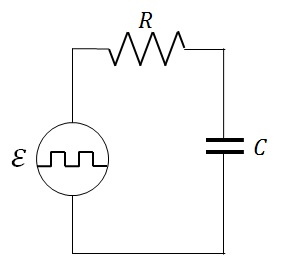
\includegraphics[scale=0.7]{Circuito-RC}
  \caption{Circuito RC con una fuente de onda cuadrada}
  \label{fig:RC}
\end{figure}

El objetivo fue medir la carga y descarga del capacitor $C$, y la corriente sobre la resistencia $R$ para obtener el tiempo característico $\tau_{RC}$ del circuito determinado por (\textbf{ecucaciones de RC}).
 
Con el fin de recrear el efecto de la $llave$ $ideal$ se programó la fuente para que emitiera una señal cuadrada con un voltaje $\varepsilon = (2.00 \pm 0.02)V$  cuya frecuencia era variable.

Para medir la diferencia de tension se conectó un osciloscopio  en paralelo al elemento que se quería medir, como se puede ven en la \textbf{Figura \ref{fig:RC}} donde muestra el caso de la resistencia. A su vez, el generador de funciones estaba conectado al osciloscopio para poder visualizar la forma funcional de la fuente. Se lo utilizó además como \texit{trigger externo} para por apreciar que tanto su señal como la caida de potencial en el elemento se encontraban en fase. Y utilizando un software de recopilación de datos se pudo importar a una computadora las mediciones registradas por el osciloscopio para ser analizadas posteriormente. Este proceso se realizó para disintos valores de $R$, considerandose despreciable la resistencia aportada por $C$ 

\subsection{Circuito RL}

De manera análoga, la siguiente parte del trabajo consistió en caracterizar un circuito RL. En este caso se reemplazo el capacitor $C$ por una inductancia $L = (1.000 \pm 0.002) H$. La forma del circuito se puede ver en la \textbf{Figura \ref{fig:RL}}.

\begin{figure}[h]
\centering
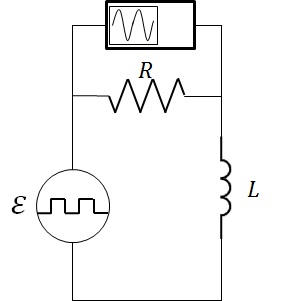
\includegraphics[scale=0.7]{Circuito-RL}
  \caption{Circuito RL con una fuente de onda cuadrada}
  \label{fig:RL}
\end{figure}

El método utilizado para obtener el tiempo característico $\tau_{RL}$, determinado por (\textbf{Ecuaciones de RL}), fue el mismo que para el circuito RC exceptuando el voltaje entregado por la fuente cuyo valor fue $(8.00 \pm 0.08) V$ y  la resistencia de la inductancia $(294 \pm 3) \Omega$, que en este caso no pudo ser despreciada, debió sumarse a la resistencia $R$ pues estaba en serie.

\subsection{Circuito RCL}

Por ultimo, se buscó estudiar el comportamiento de un circuito RCL. Para ello se montó un circuito cerrado que tenia en serie la fuente programable $\varepsilon$, la resistencia variable por decadas $R$, una inductancia variable $L$ y un capacitor $C$ como muestra la \textbf{Figura \ref{fig:RCL}}.  

\begin{figure}[h]
\centering
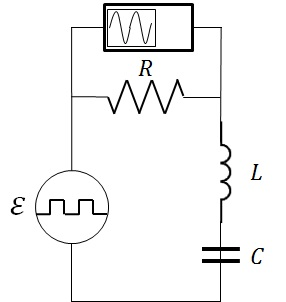
\includegraphics[scale=0.7]{Circuito-RCL}
  \caption{Circuito RCL con una fuente de onda cuadrada}
  \label{fig:RCL}
\end{figure}

Para caracterizar el circuito, la ecuación (\textbf{ecuaciones de RCL}) determina distintos regímenes de comportamiento que depende de los parámetros que se usen.

Utilizando el método de adquisición de datos ya explicado, se midió la diferencia de potencial sobre la resistencia. Esta diferencia de potencial era generada por una señal cuadrada de $(3.08 \pm 0.04)V$.

Por lo tanto se estudió el circuito para disintos valores de $R$,$C$ y $L$ con el fin de encontrar cada uno de estos regímenes.
%%%%%%%%%%%%%%%%%%%%%%%%%%%%%%%%%%%%%%%%%%%%%%%%%%%%%%%%%%%%%%%%%%%%%%%%%%%%%%%%%%%%%%%%%%%%%%%%%%%%%%%%%%%%%%%%%%%%%%%%%%%%%%%%
% 4.DISCUSIÓN Y RESULTADOS: todo lo que se obtuvo y explicación. Graficos, tablas.
%%%%%%%%%%%%%%%%%%%%%%%%%%%%%%%%%%%%%%%%%%%%%%%%%%%%%%%%%%%%%%%%%%%%%%%%%%%%%%%%%%%%%%%%%%%%%%%%%%%%%%%%%%%%%%%%%%%%%%%%%%%%%%%%

\section{Resultados}
\label{sec:discusion}

\subsection{Circuito RC}


\subsection{Circuito RL}


\subsection{Circuito RCL}



%%%%%%%%%%%%%%%%%%%%%%%%%%%%%%%%%%%%%%%%%%%%%%%%%%%%%%%%%%%%%%%%%%%%%%%%%%%%%%%%%%%%%%%%%%%%%%%%%%%%%%%%%%%%%%%%%%%%%%%%%%%%%%%%
%	CONCLUSIONES
%%%%%%%%%%%%%%%%%%%%%%%%%%%%%%%%%%%%%%%%%%%%%%%%%%%%%%%%%%%%%%%%%%%%%%%%%%%%%%%%%%%%%%%%%%%%%%%%%%%%%%%%%%%%%%%%%%%%%%%%%%%%%%%%

\section{Conclusiones}
\label{sec:conclusiones}




%%%%%%%%%%%%%%%%%%%%%%%%%%%%%%%%%%%%%%%%%%%%%%%%%%%%%%%%%%%%%%%%%%%%%%%%%%%%%%%%%%%%%%%%%%%%%%%%%%%%%%%%%%%%%%%%%%%%%%%%%%%%%%%%%
%	APÉNDICE: esas cosas extras que simplemente no tuvieron lo suficiente como para ganarse una sección propia.
%%%%%%%%%%%%%%%%%%%%%%%%%%%%%%%%%%%%%%%%%%%%%%%%%%%%%%%%%%%%%%%%%%%%%%%%%%%%%%%%%%%%%%%%%%%%%%%%%%%%%%%%%%%%%%%%%%%%%%%%%%%%%%%%%



%%%%%%%%%%%%%%%%%%%%%%%%%%%%%%%%%%%%%%%%%%%%%%%%%%%%%%%%%%%%%%%%%%%%%%%%%%%%%%%%%%%%%%%%%%%%%%%%%%%%%%%%%%%%%%%%%%%%%%%%%%%%%%%%%
%	REFERENCIAS: libros, libros, libros.
%%%%%%%%%%%%%%%%%%%%%%%%%%%%%%%%%%%%%%%%%%%%%%%%%%%%%%%%%%%%%%%%%%%%%%%%%%%%%%%%%%%%%%%%%%%%%%%%%%%%%%%%%%%%%%%%%%%%%%%%%%%%%%%%%

%Ejemplo:
\begin{thebibliography}{1}
 \bibitem{Berkeley} Frank S. Crawford, \textit{Berkeley physics course 3: Ondas}, 1994, Editorial Reverte S.A.
\end{thebibliography}
%Para citar: blablabla \cite{Baird}
 
\end{document}





